\documentclass[11pt,a4paper]{article}
\usepackage[utf8]{inputenc}
\usepackage[spanish]{babel}
\usepackage{amsmath}
\usepackage{amsfonts}
\usepackage{amssymb}
\usepackage{graphicx}
\usepackage{enumitem}
\usepackage{geometry}
\usepackage{float}

\geometry{left=2.5cm,right=2.5cm,top=2.5cm,bottom=2.5cm}

\begin{document}

\begin{center}
    \textbf{UNIVERSIDAD TECNOLÓGICA NACIONAL \\ FACULTAD REGIONAL LA PLATA} \\
    \vspace{0.2cm}
    \textbf{INGENIERÍA CIVIL — Curso 2026} \\
    \vspace{0.2cm}
    \textit{Asignatura: ESTABILIDAD}
\end{center}

\vspace{0.3cm}

\begin{flushleft}
    \textbf{Prof. Titular:} Ing. Daniel Zangara \\
    \textbf{JTP:} Ing. Jorge Ronconi \\
\end{flushleft}

\noindent\rule{\linewidth}{0.4pt}

\begin{center}
    \vspace{0.4cm}
    \Large \textbf{Trabajo Práctico N$^\circ$4:\\ SISTEMAS DE FUERZAS EN EL ESPACIO} \\
    \vspace{0.4cm}
\end{center}

% --- EJERCICIO 1 ---
\subsection*{Ejercicio N$^\circ$1: Mástil con dos cables y un puntal}

Un mástil vertical $AB$ se apoya en una rótula en $A(0,0,0)$ y su extremo
superior se ubica en $B(0,0,6)$ m. En el punto $B$ convergen dos cables
$BD$ y $BE$ que se anclan en el plano horizontal, y el puntal $AB$.
Las coordenadas de los puntos de anclaje son:

\begin{center}
\begin{tabular}{cccc}
\hline
\textbf{Punto} & $x$ [m] & $y$ [m] & $z$ [m] \\
\hline
$A$ & 0 & 0 & 0 \\
$B$ & 0 & 0 & 6{,}0 \\
$D$ & $-2{,}0$ & $3{,}0$ & 0 \\
$E$ & $-3{,}0$ & $-3{,}0$ & 0 \\
\hline
\end{tabular}
\end{center}

En el punto $B$ se aplica una fuerza de módulo $P = 12\,\text{kN}$, inclinada $20^\circ$ respecto a la horizontal y contenida en un plano que forma $-45^\circ$ con el plano $YZ$ (sentido horario visto desde el eje $Z$ positivo).

Los cables $BD$ y $BE$ solo pueden transmitir tracción.
El puntal $AB$ puede transmitir tracción o compresión.

\begin{enumerate}[label=\alph*)]
    \item Determinar las fuerzas en los cables $T_{BD}$ y $T_{BE}$ y en el puntal $F_{AB}$ planteando tres ecuaciones de equilibrio de fuerzas en el nudo $B$.
    \item Indicar si cada elemento trabaja a tracción o compresión y verificar que el resultado es físicamente admisible para los cables.
    \item Determinar las reacciones en la rótula $A$: $R_{Ax}$, $R_{Ay}$ y $R_{Az}$.
\end{enumerate}

\begin{figure}[H]
    \centering
    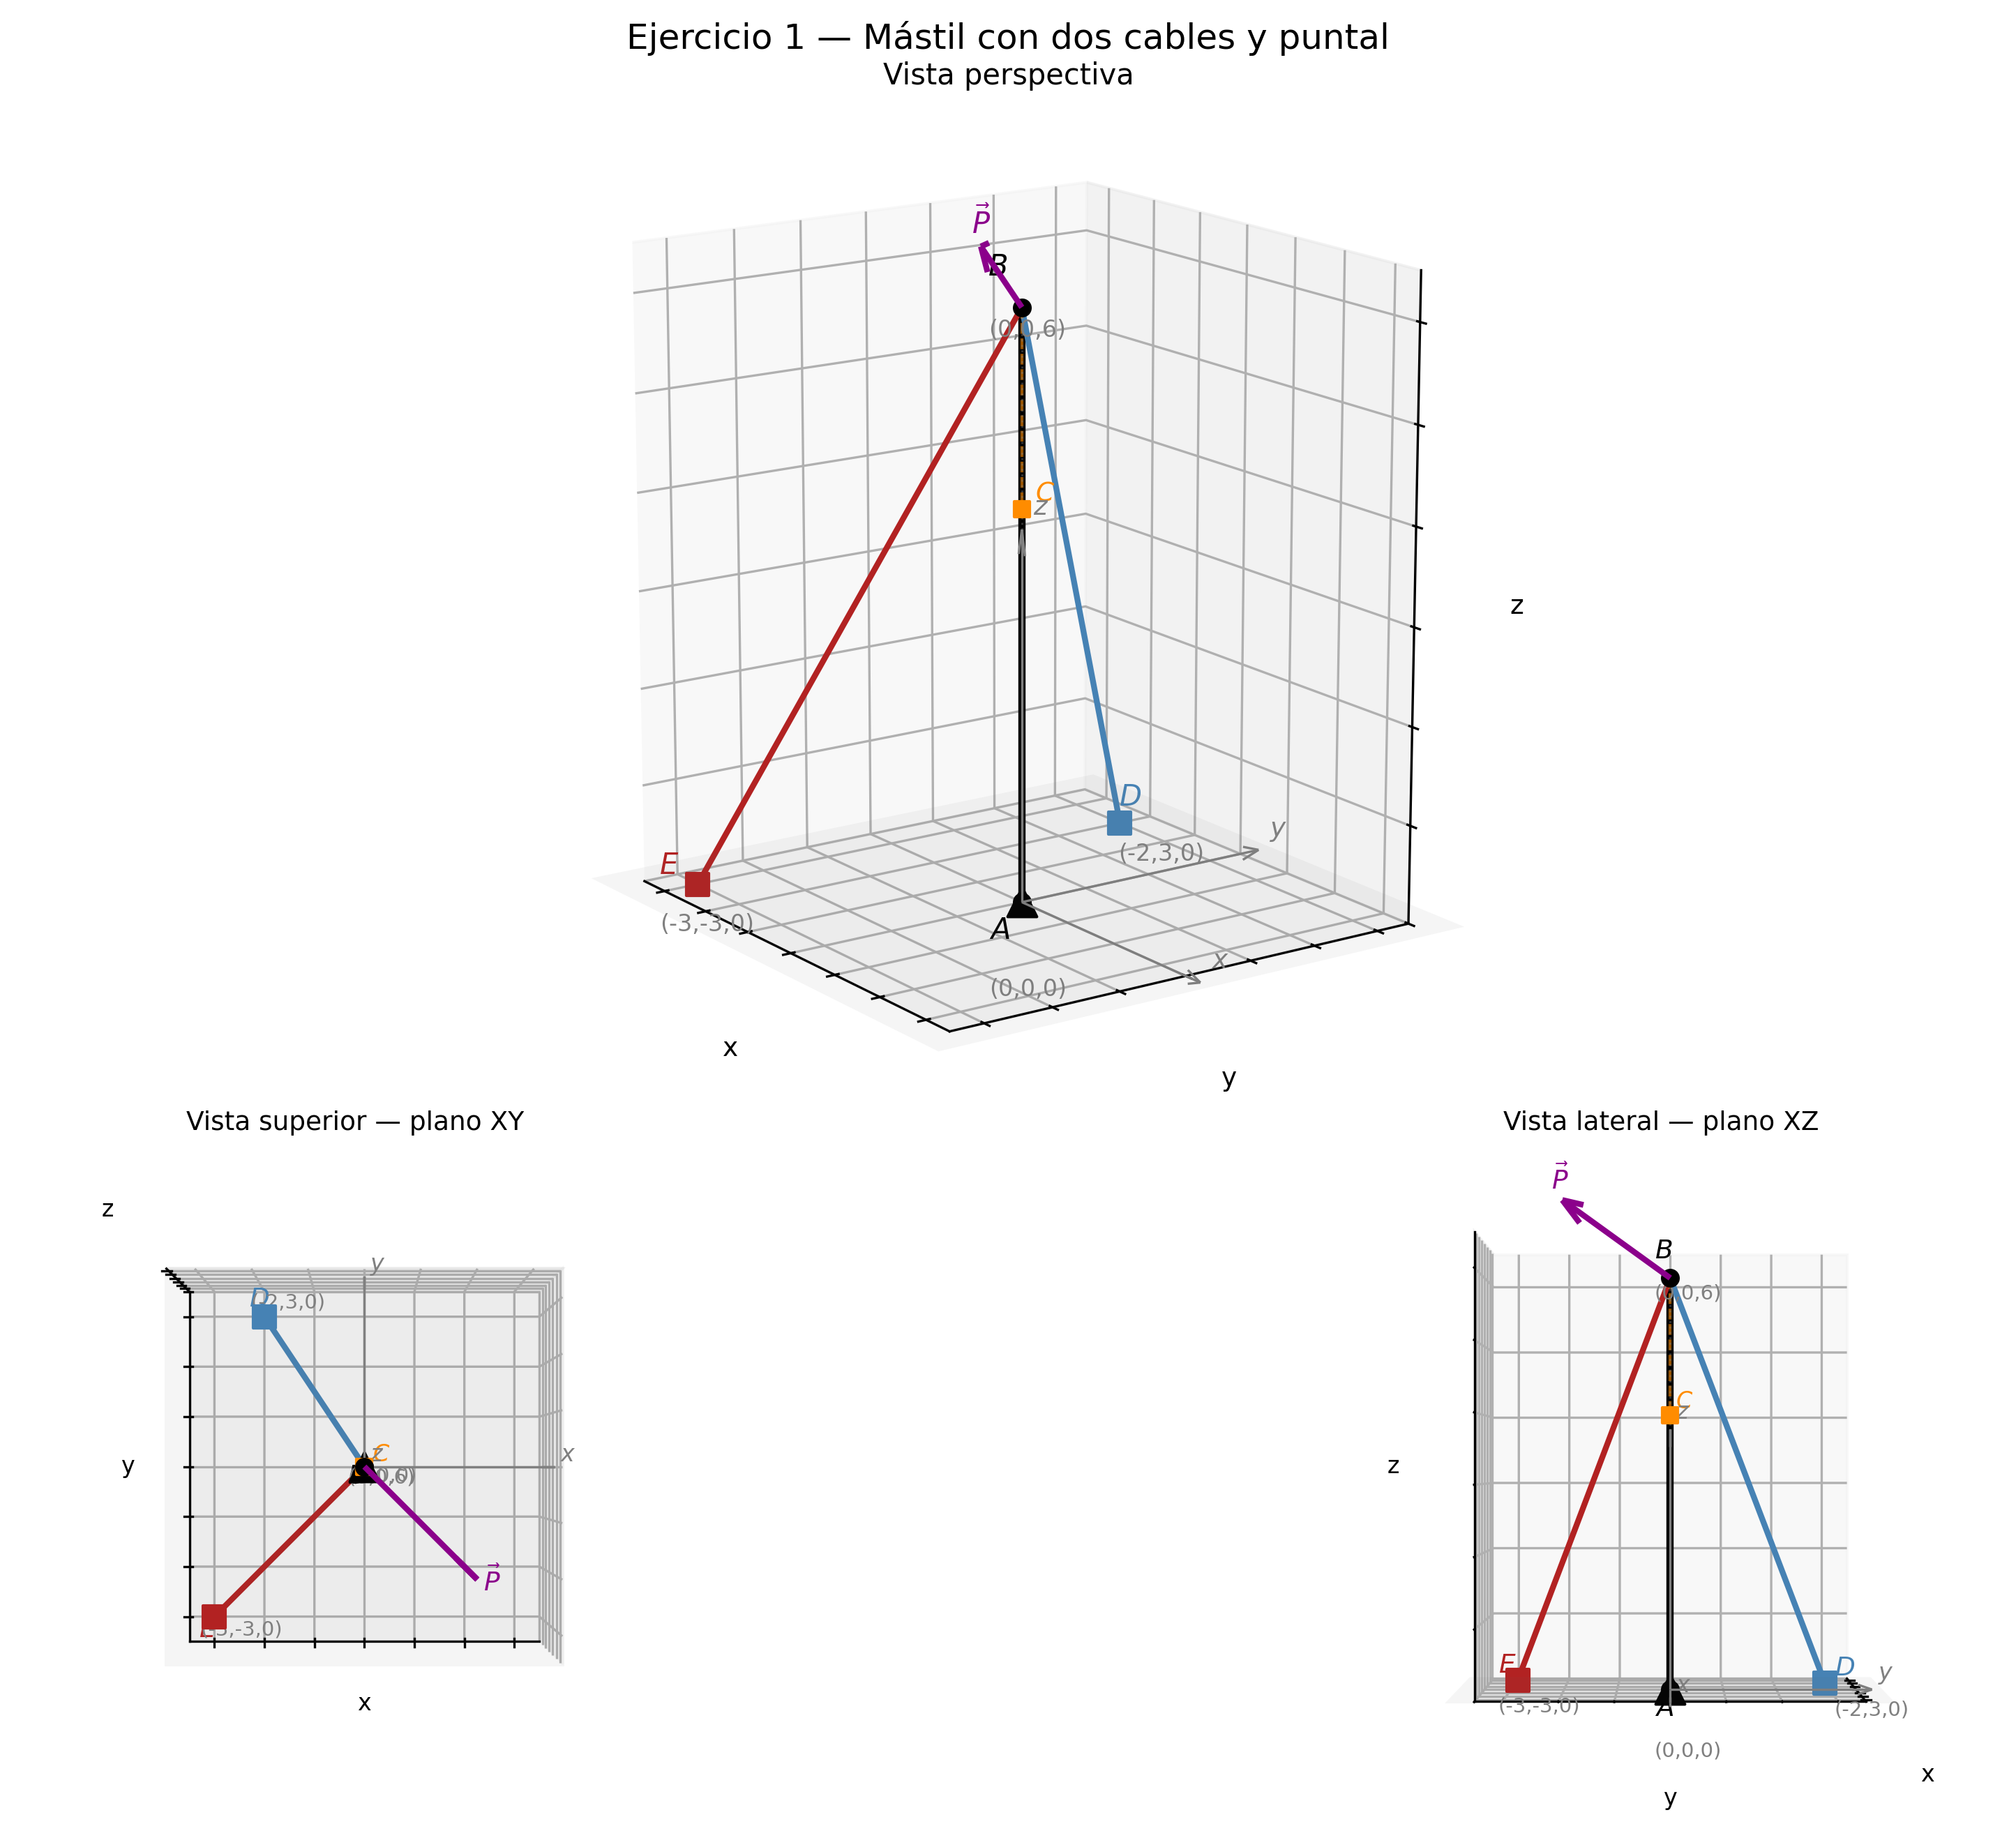
\includegraphics[width=0.90\textwidth]{img/tp4_ej1.png}
    \caption{Mástil con dos cables y un puntal — Ejercicio 1.}
    \label{fig:tp4ej1}
\end{figure}

\noindent\rule{\linewidth}{0.4pt}

% --- EJERCICIO 3 ---

\subsection*{Ejercicio N$^\circ$3: Cartel prismático con columnas y cables}

Un cartel publicitario tiene forma de prisma rectangular de $a = 5{,}0\,\text{m}$ de ancho, $h = 3{,}0\,\text{m}$ de alto y $e = 0{,}30\,\text{m}$ de espesor. Está soportado por dos columnas verticales de sección $0{,}30\,\text{m} \times 0{,}30\,\text{m}$ ubicadas en las esquinas inferiores $A$ y $B$, y estabilizado por cuatro cables que parten de las esquinas superiores $C$ y $D$ hacia puntos de anclaje en el terreno.

Las coordenadas del sistema son:

\begin{center}
\begin{tabular}{cccc}
\hline
\textbf{Punto} & $x$ [m] & $y$ [m] & $z$ [m] \\
\hline
$A$ & 0 & 0 & 0 \\
$B$ & 5{,}0 & 0 & 0 \\
$C$ & 0 & 0 & 3{,}0 \\
$D$ & 5{,}0 & 0 & 3{,}0 \\
\hline
\end{tabular}
\end{center}

Desde cada esquina superior ($C$ y $D$) parten dos cables simétricos,
formando $45^\circ$ en planta (respecto al eje $y$) y $30^\circ$ con
la vertical. Los cuatro anclajes en el terreno tienen las siguientes
coordenadas:

\begin{center}
\begin{tabular}{cccc}
\hline
\textbf{Anclaje} & $x$ [m] & $y$ [m] & $z$ [m] \\
\hline
$E$ & $-d$ & $-d$ & 0 \\
$F$ & $-d$ & $+d$ & 0 \\
$G$ & $5{,}0+d$ & $-d$ & 0 \\
$H$ & $5{,}0+d$ & $+d$ & 0 \\
\hline
\end{tabular}
\end{center}

donde $d = h \cdot \tan30^\circ \cdot \cos45^\circ =
3{,}0 \times 0{,}577 \times 0{,}707 = 1{,}225\,\text{m}$.

La presión de diseño del viento es $p_w = 1{,}0\,\text{kN/m}^2$,
actuando normalmente sobre la cara frontal del cartel
($5{,}0 \times 3{,}0\,\text{m}^2$).
El peso propio del cartel es $W = 4{,}0\,\text{kN}$, actuando
en el centroide de la cara frontal.
El peso propio de cada columna es $W_c = 0{,}5\,\text{kN}$.

\begin{enumerate}[label=\alph*)]
    \item Calcular las coordenadas de los anclajes $E$, $F$, $G$ y $H$
    a partir del ángulo de $30^\circ$ con la vertical y $45^\circ$
    en planta. Verificar que todos los cables tienen la misma longitud.
    \item Calcular la fuerza resultante de viento $F_w$ y su punto
    de aplicación (centroide de la cara frontal).
    \item Plantear el equilibrio del sistema determinando las tensiones
    en los cuatro cables $T_E$, $T_F$, $T_G$ y $T_H$, y las fuerzas
    axiales en las columnas $N_A$ y $N_B$.
    \item Verificar el equilibrio global:
    $\sum F_x = 0$, $\sum F_z = 0$, $\sum M = 0$.
    \item Indicar qué cables trabajan más y por qué, considerando
    la acción simultánea del peso y el viento.
\end{enumerate}

\textbf{Datos:}
\begin{itemize}
    \item Dimensiones del cartel: $a = 5{,}0\,\text{m}$,
    $h = 3{,}0\,\text{m}$, $e = 0{,}30\,\text{m}$
    \item Sección columnas: $0{,}30\,\text{m} \times 0{,}30\,\text{m}$
    \item Ángulo de cables con la vertical: $30^\circ$
    \item Ángulo de cables en planta: $45^\circ$
    \item Presión de viento: $p_w = 1{,}0\,\text{kN/m}^2$
    \item Peso propio cartel: $W = 4{,}0\,\text{kN}$
    \item Peso propio cada columna: $W_c = 0{,}5\,\text{kN}$
    \item Los cables solo trabajan a tracción
\end{itemize}

\begin{figure}[H]
    \centering
    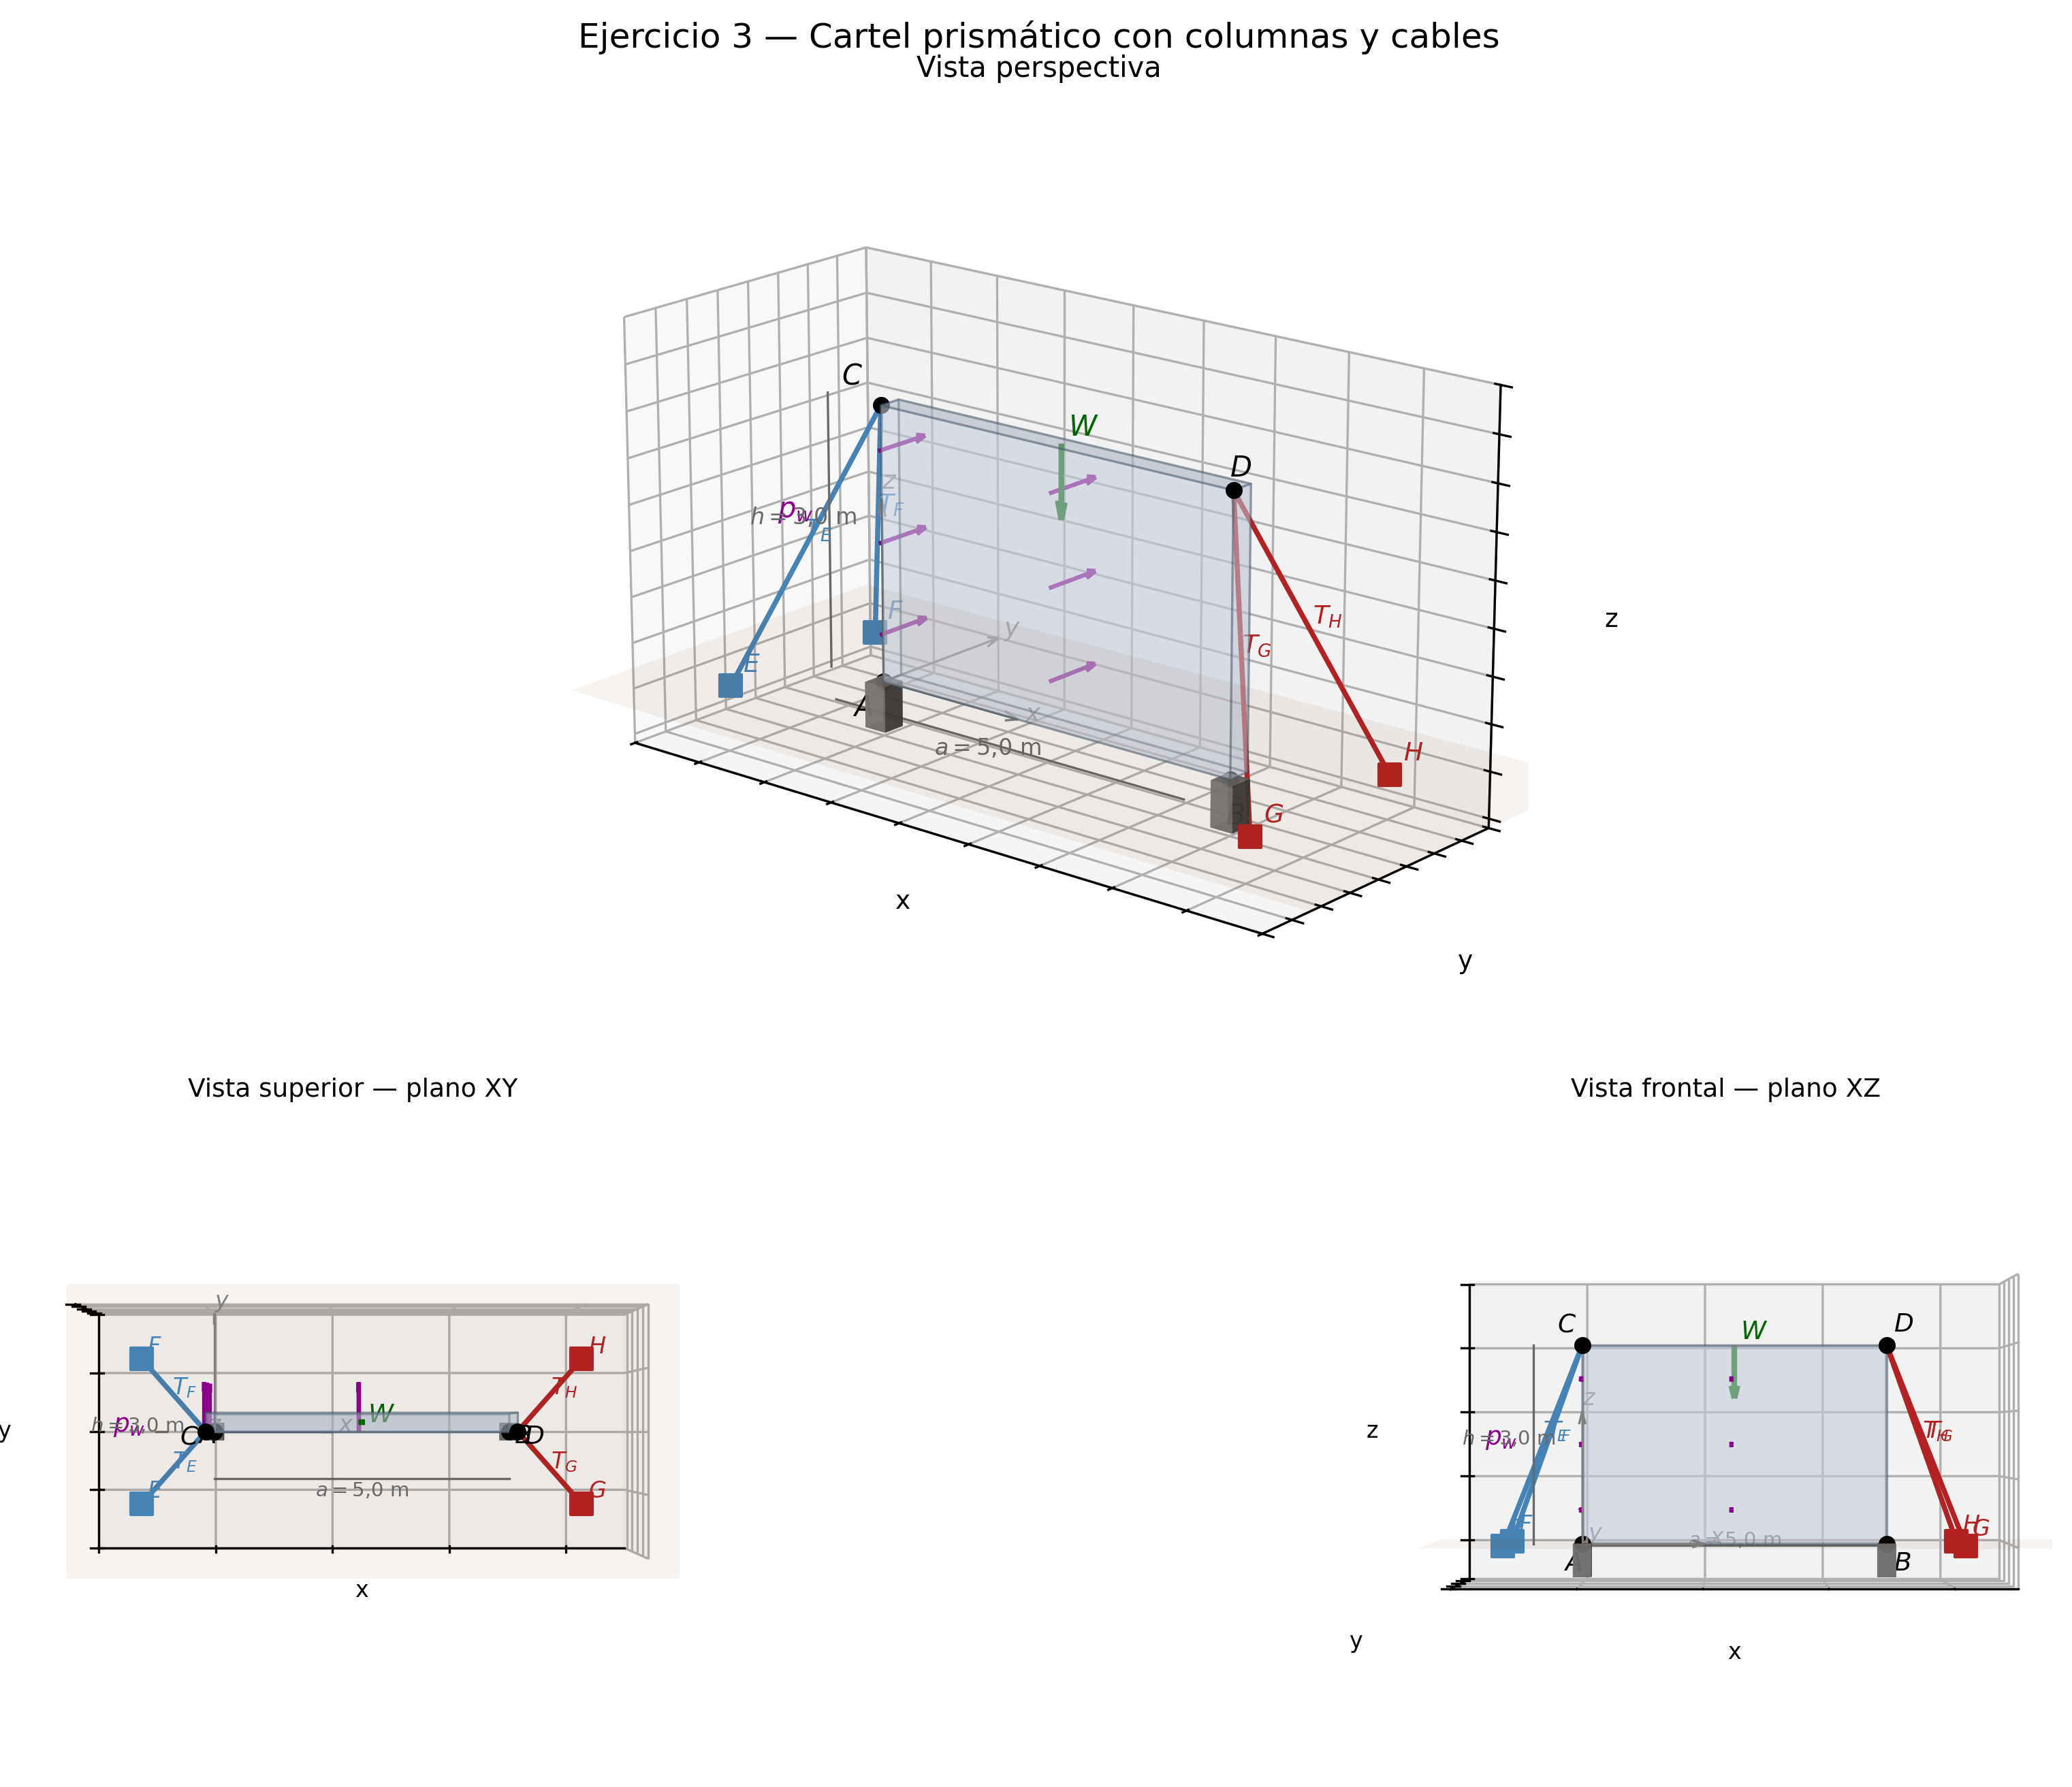
\includegraphics[width=0.70\textwidth]{img/tp4_ej3.png}
    \caption{Viga en voladizo con cables — Ejercicio 2.}
    \label{fig:tp4ej2}
\end{figure}

\noindent\rule{\linewidth}{0.4pt}

% --- EJERCICIO 4 ---
\subsection*{Ejercicio N$^\circ$4: Placa rectangular}

Una placa rectangular $ABCD$ de dimensiones $a = 3{,}0\,\text{m}$ y $b = 2{,}0\,\text{m}$ y peso $P = 8\,\text{kN}$ está sostenida horizontalmente por tres barras verticales articuladas en los puntos $E$, $F$ y $G$ (ver Figura~3). Las coordenadas de los puntos de apoyo son:

\begin{center}
\begin{tabular}{cccc}
\hline
\textbf{Punto} & $x$ [m] & $y$ [m] & Descripción \\
\hline
$E$ & 0 & 0 & Vértice $A$ \\
$F$ & 3{,}0 & 0 & Vértice $B$ \\
$G$ & 0 & 2{,}0 & Vértice $C$ \\
\hline
\end{tabular}
\end{center}

Adicionalmente, se aplica una carga puntual $Q = 4\,\text{kN}$ hacia abajo
en el punto $H(2{,}0;\,1{,}5)$ m del plano de la placa.

\begin{enumerate}[label=\alph*)]
    \item Determinar las fuerzas en las tres barras $P_E$, $P_F$ y $P_G$
    planteando una ecuación de sumatoria de fuerzas verticales y dos
    ecuaciones de momentos respecto a los ejes.
\end{enumerate}

\begin{figure}[H]
    \centering
    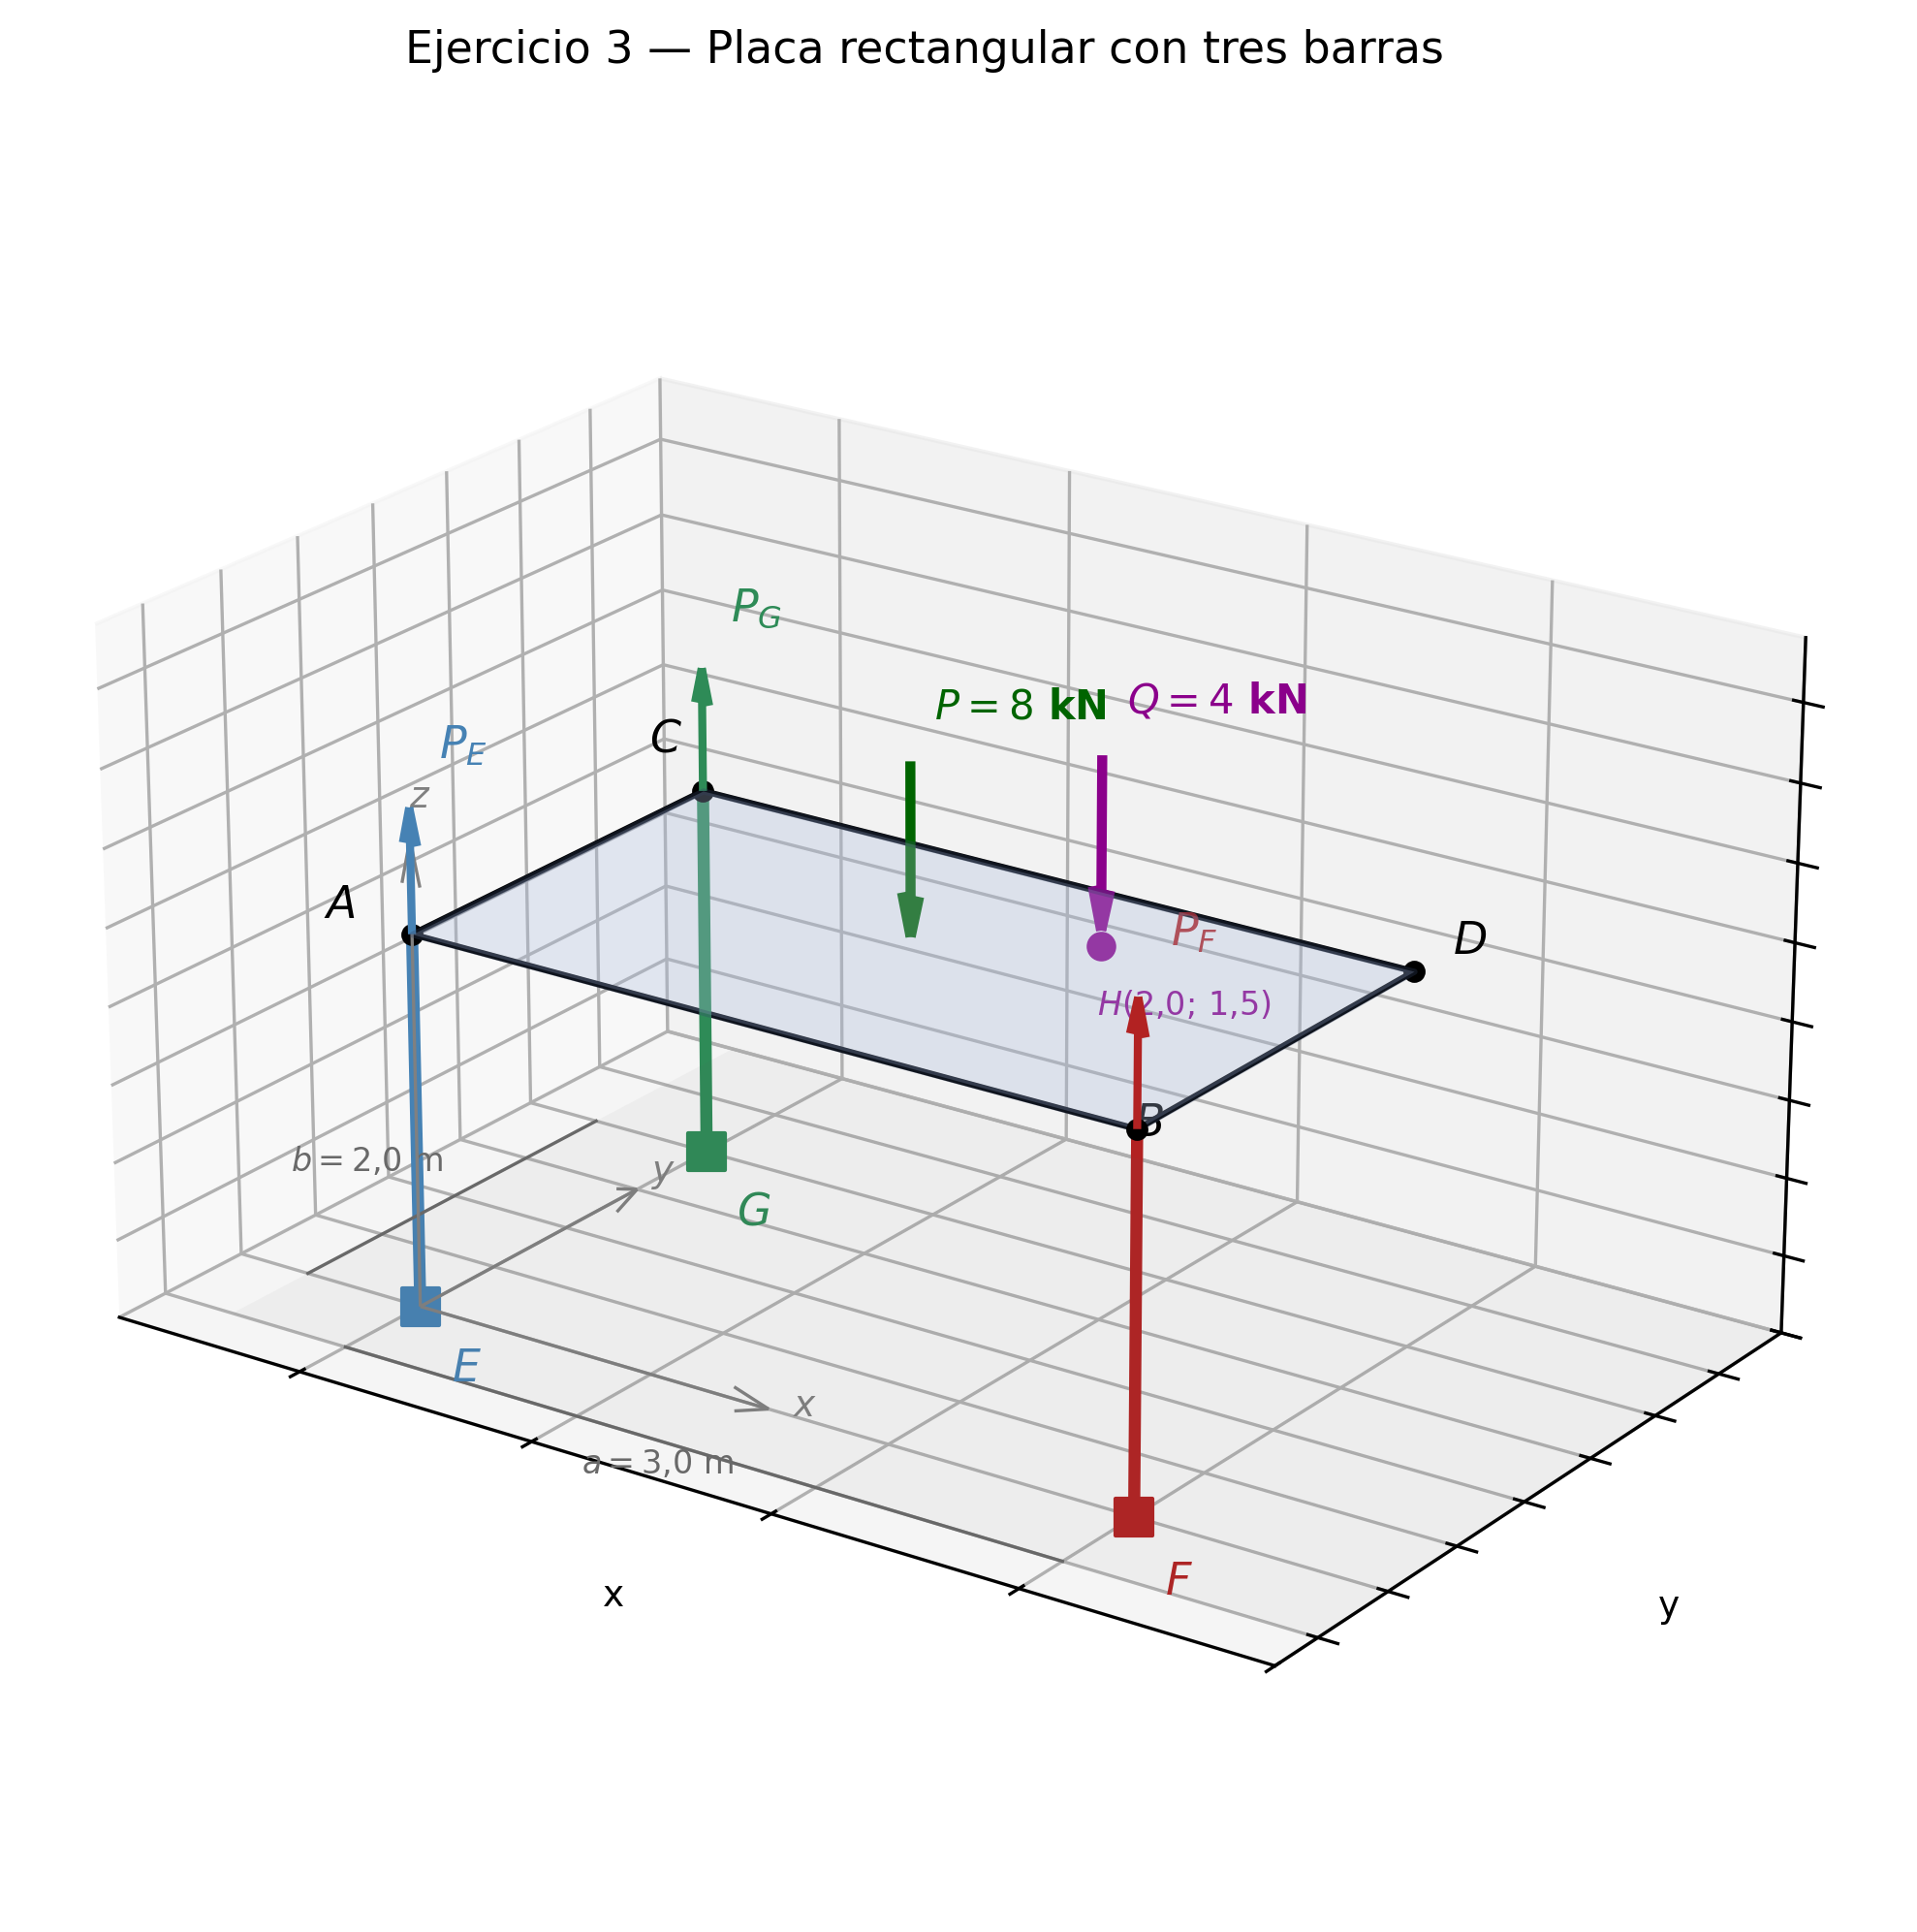
\includegraphics[width=0.70\textwidth]{img/tp4_ej4.png}
    \caption{Placa rectangular sostenida por tres barras — Ejercicio 3.}
    \label{fig:tp4ej3}
\end{figure}

\noindent\rule{\linewidth}{0.4pt}

% --- EJERCICIO 5 ---
\subsection*{Ejercicio N$^\circ$5: Cilindro con polea y contrapeso}

Un cilindro de radio $R = 0{,}25\,\text{m}$ tiene su eje horizontal $AB$
apoyado en dos cojinetes ubicados en $A$ y $B$, separados $L = 1{,}00\,\text{m}$
entre sí. Los cojinetes solo pueden transmitir reacciones en $y$ y en $z$.
Una cuerda enrollada en el cilindro sostiene una carga $Q = 4\,\text{kN}$
que cuelga verticalmente a un lado del cilindro a $0{,}50\,\text{m}$ de $A$.
Una polea ubicada en el punto $C$ a $0{,}30\,\text{m}$ de $A$ como muestra la figura.

\begin{enumerate}[label=\alph*)]
    \item Determinar la magnitud de la fuerza $P$ necesaria para mantener
    el equilibrio del sistema planteando la ecuación de momentos respecto
    al eje $AB$.
    \item Determinar las reacciones en los cojinetes $A$ y $B$:
    $Y_A$, $Z_A$, $Y_B$ y $Z_B$ planteando las ecuaciones de equilibrio restantes.
\end{enumerate}

\begin{figure}[H]
    \centering
    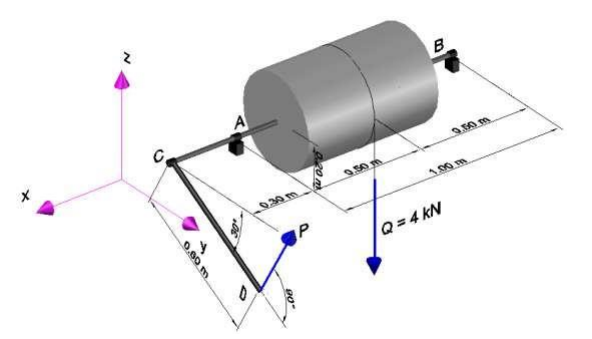
\includegraphics[width=0.70\textwidth]{img/tp4_ej5.png}
    \caption{Cilindro con polea y contrapeso — Ejercicio 4.}
    \label{fig:tp4ej4}
\end{figure}

\end{document}